\subsection{Simulation of DGPs}
\textbf{\textit{\begin{itemize}
  \item[a)] Generate a realization of a Gaussian stochastic process of sample size T = 500, and plot the time series against time
\end{itemize}}}\noindent
As the data generating process (DGP) is stochastic without any autoregressive element, we simply perform 500 draws from a standard normal distribution. Panel A in figure \ref{fig:gaussian} shows the sime series, whereas the histogram in panel B confirms that the realizations are approximately standard normal distributed.
\begin{figure}[H]
  \caption{Gaussian stochastic process}
  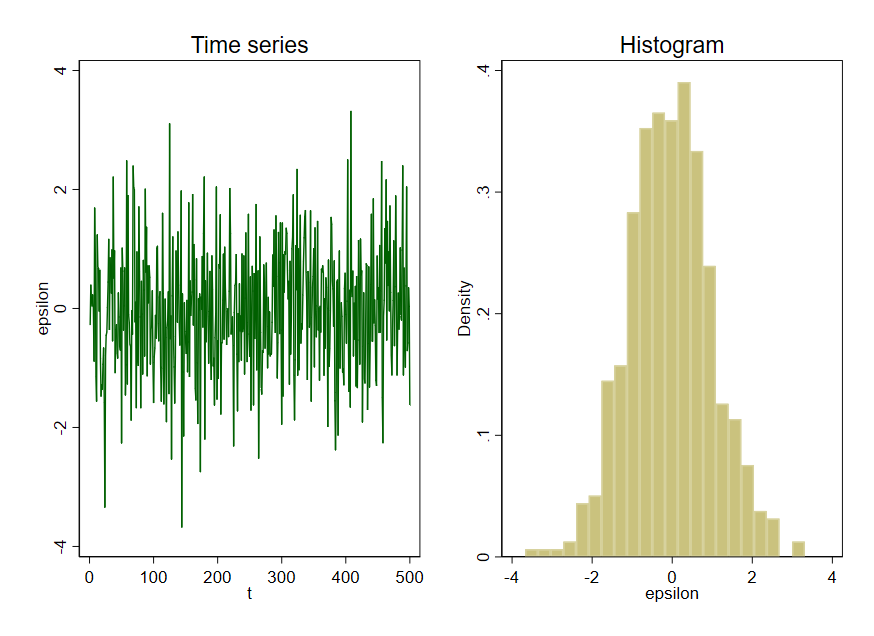
\includegraphics[width= \textwidth]{03_figures/fig22a}
  \label{fig:gaussian}
  \vspace{-2cm}
\end{figure}
\textbf{\textit{\begin{itemize}
  \item[b)] Generate AR(1) processes with three different autoregressive coefficients $\bm{\phi=\{0.5,0.8,0.95\}}$
\end{itemize}}}\noindent
Keeping the sample size at 500 and including a burn-in period of 2.000 iterations, the time series for the autoregressive models are plotted in figure \ref{fig:ar1}. The autocorrelation functions (ACFs) and partial autocorrelation functions (PACFs) are plottes in figure \ref{fig:ar1_acf}.
\\ \\
While all three processes are mean-reverting as the stationarity condition $|\phi|<1$ is fulfilled, it is clear that persistence increases as $\phi\rightarrow1$. This translates into longer lasting and more extreme cycles in figure \ref{fig:ar1} as the autoregressive element dominates the stochastic error term. Likewise, the ACFs in figure \ref{fig:ar1_acf} show that temporal dependence is significant three periods back for $\phi=0.5$ while the autocorrelation is significant for the past 12-13 periods for $\phi=0.95$. While I have only shown 25 lags in the figures, extending it even shows that the latter process is near-borderline significantly autocorrelated with period 30-37 as well, but negatively.

Figure \ref{fig:ar1_acf} shows for the ACFs as well as for the PACFs that the coefficient of correlation with the first lag is close to the actual $\phi$-values in the DGP. Except for a few outliers, the PACFs are inconsistent with AR(p) models of order $p>1$.

Furthermore, the number of lags that are significantly autocorrelated are much higher in the ACFs as opposed to the PACFs this indicate that the processes are AR(1) and not MA(q) or ARMA(1,q) processes.
\begin{figure}[H]
  \caption{AR(1) processes with different autocorrelation coefficients}
  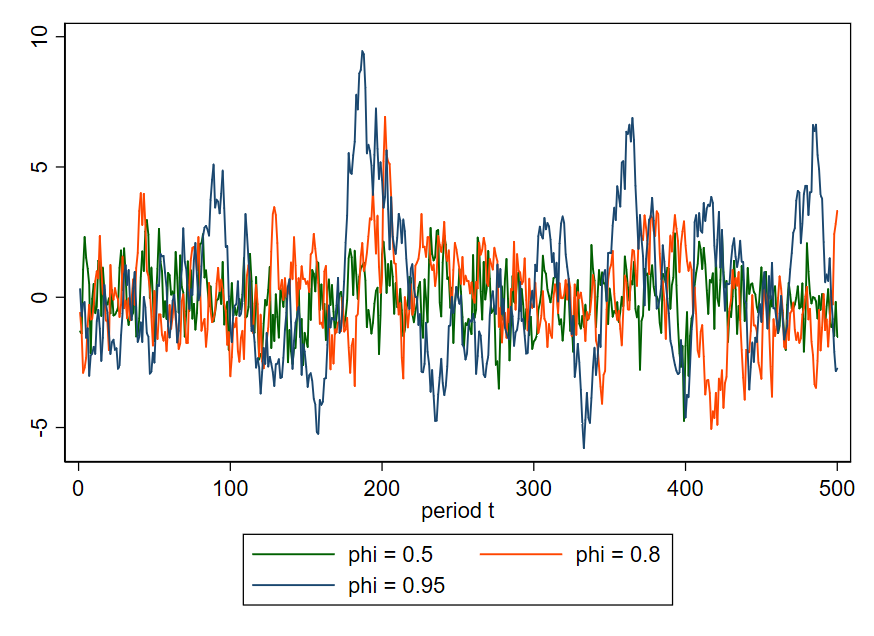
\includegraphics[width= \textwidth]{03_figures/fig22b}
  \label{fig:ar1}
  \vspace{-1cm}
\end{figure}
\begin{figure}[H]
  \caption{Autocorrelation and Partial Autocorrelation functions for AR(1) processes}
  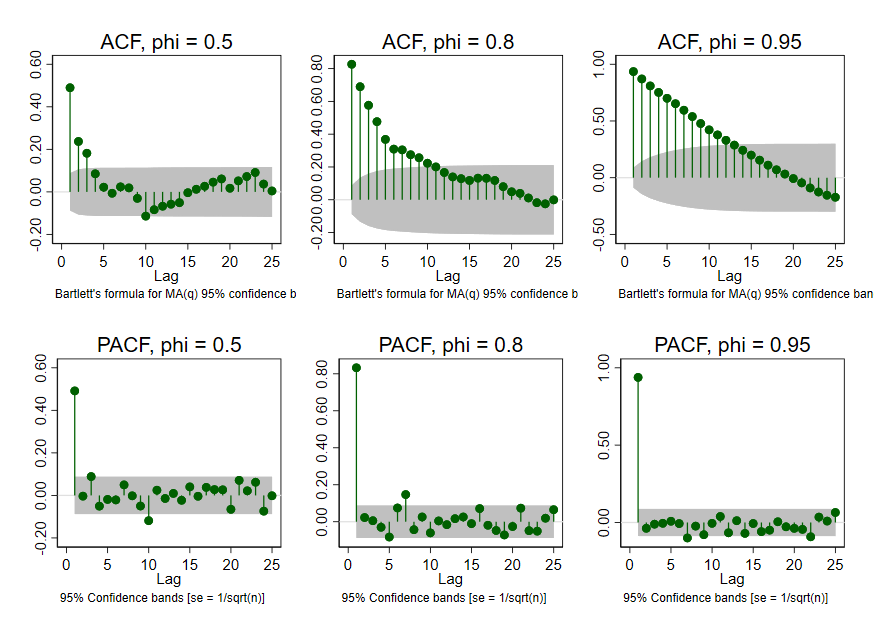
\includegraphics[width= \textwidth]{03_figures/fig22b_ac}
  \label{fig:ar1_acf}
  \vspace{-1cm}
\end{figure}
% MA(1)
\textbf{\textit{\begin{itemize}
  \item[b)] Generate MA(1) processes with three different moving average coefficients $\bm{\theta=\{0.5,0.8,0.95\}}$
\end{itemize}}}\noindent
The Moving Average processes are likewise generated with a sample size of 500 including a burn-in period of 2.000 iterations. The time series are plotted in figure \ref{fig:ma1} and the autocorrelation functions and partial autocorrelation functions are plottes in figure \ref{fig:ma1_acf} on the next page.
\\ \\
As opposed to the AR(1) processes there are as good as no signs of persistence in the time series for the MA(1) processes. Though a bit difficult to tell from comparison of figure \ref{fig:gaussian} and \ref{fig:ma1}, the summary statistics show that the standard deviation is a little higher for the MA(1) processes than for the standard normal distribution, and increase slightly with $\theta\rightarrow1$. This is due to an increased persistence of prior shocks.

The ACFs in figure \ref{fig:ma1_acf} confirms that there are not any persistence after the 1st lag, while the PACFs show significant lags besides the first but with alternating sign. For $\theta=0.5$ $x_t$ is linearly correlated with $x_{t-1},\ x_{t-2},$ and $x_{t-3}$ and arguably with $x_{t-4}$ (borderline significant). The MA(1) process with $\theta=0.95$ on the other hand shows significant correlation with all lags 1-8.

The number of significant lags are much higher in the PACFs as opposed to the ACFs where only the first lag is significant which is consistent with an MA(q) model of order $q=1$ while inconsistent with the processes being AR(p) or ARMA(p,q) processes.
\begin{figure}[H]
  \caption{MA(1) processes with different autocorrelation coefficients}
  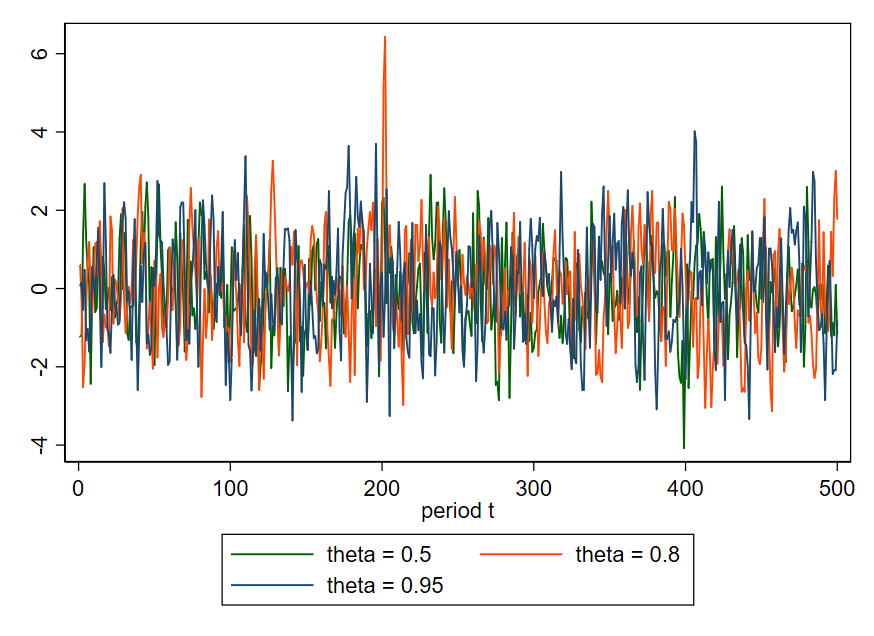
\includegraphics[width= \textwidth]{03_figures/fig22c}
  \label{fig:ma1}
  \vspace{-0.1cm}
\end{figure}
\begin{figure}[H]
  \vspace{-1cm}
  \caption{Autocorrelation and Partial Autocorrelation functions for MA(1) processes}
  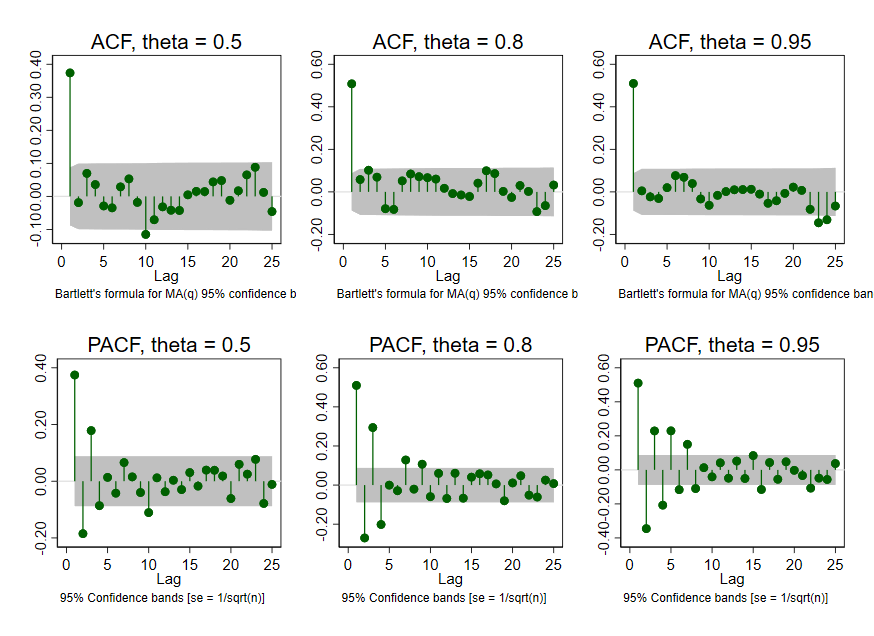
\includegraphics[width= \textwidth]{03_figures/fig22c_ac}
  \label{fig:ma1_acf}
  \vspace{-1cm}
\end{figure}
